\documentclass[10pt,a4paper,oneside]{book}

\usepackage[slovene]{babel}
\usepackage[utf8x]{inputenc}
\usepackage{makeidx}
\usepackage{graphicx}
\usepackage{enumerate}
\usepackage[margin=1in]{geometry}
\usepackage{verbatim}
\usepackage[svgnames]{xcolor}
\usepackage{fancybox}
\usepackage{varwidth}
\newcommand\inline[1]{%
\begin{Sbox}{#1}\end{Sbox}%
\colorbox{lightgray}{\TheSbox}%
}
\newcommand\inliney[1]{%
\begin{Sbox}\begin{varwidth}{0.91\textwidth}{#1}\end{varwidth}\end{Sbox}%
\colorbox{lightgray}{\TheSbox}%
}

\newcommand\pic[2]{%
\parbox{1cm}{%
\begin{center}%
\includegraphics[width=#1\textwidth]{#2}%
\end{center}%
}%
}

\newcommand\br{%
 \ \\ \ \\%
}

\usepackage{hyperref}
\hypersetup{
    colorlinks=true,
    linkcolor=black,
    urlcolor=blue,
    pdftitle={AngryPigs}
}
\title{AngryPigs}

\begin{document}
\begin{titlepage}
\begin{center}
\ \\[3.5cm]
{\resizebox{16.8cm}{!}{\Huge\bf\color{LightGreen}\texttt{AngryPigs{\tiny\ }}}}\\[-2.8cm]
{\resizebox{16.8cm}{!}{\Huge\bf\color{Green}\texttt{{\tiny\ }AngryPigs}}}\\[3.9cm]
{\Huge\bf Dokumentacija}\\[0.35cm]
{\huge\today}\ \\[4.5cm]
{\Huge {\bf Avtorja}}\\[0.35cm]
{\huge Matic Potočnik, Jaka Sivec}
\vfill
\end{center}
\end{titlepage}
\chapter{O igri}
Angry Pigs je zabavna 3D igra, v kateri igralec obstreljuje drevesa in skuša z njih sklatiti ptiče, ter njihova gnezda. 
\br
Igra je napisana v jezikih Clojure in Scala, z uporabo OpenGL knjižnice LWJGL.
\br
\begin{center}
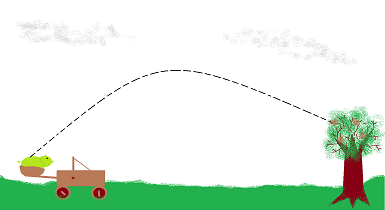
\includegraphics[width=12cm]{conceptsmall}
\end{center}

\chapter{Tehnologija}

\section{Generiranje dreves}

\section{The rest}

\chapter{Rezultati}


\end{document}